\section{Experiments}
\label{openpsg:sec:experiments}


\subsection{Datasets}

\noindent \textbf{Panoptic Scene Graph (PSG)} dataset~\cite{yang2022panoptic} is constructed based on the COCO dataset~\cite{lin2014microsoft, caesar2018coco}, consisting of 48,749 annotated images: 46,563 for training and 2,186 for testing. 
It encompasses 80 ``thing'' object categories~\cite{lin2014microsoft} and 53 ``stuff'' object categories~\cite{caesar2018coco}, as well as 56 relation categories.

\noindent \textbf{Visual Genome (VG)} dataset~\cite{krishna2017visual} is a widely used dataset in the SGG task.
To further validate our method, we follow previous works~\cite{yu2023visually, chen2023expanding} and test our method on the VG-150 variant, which contains 150 object categories and 50 relation categories.


\subsection{Tasks and Metrics}

\noindent \textbf{Tasks.}
In both PSG and SGG, there are three distinct subtasks: Predicate Classification (PredCls), Scene Graph Classification (SGCls), and Scene Graph Detection (SGDet)~\cite{xu2017scene}.
In PredCls, the categories and locations of objects within the image are given, and only the relation categories between the objects need to be predicted.
SGCls requires predicting both the categories of objects and the relations between them, given the locations of objects within the image.
SGDet requires the simultaneous prediction of object categories, locations, and relations between objects, based on the given image.
In this chapter, we focus on the PredCls and SGDet subtasks.
The PredCls excludes the influence of segmentation performance and only compares the relation prediction performance, while the SGDet considers the combined results for both object segmentation and relation prediction.

Furthermore, to validate our method's capability in open-set relation prediction, we divide the dataset into base relations and novel relations at a ratio of 7:3.
For the PSG dataset, the specific division method is provided in Appendix~C.
For the division of the VG dataset, we follow the practice in previous works~\cite{yu2023visually, chen2023expanding}.
In the open-set scenarios, our model is trained with data only from base relations and tested on both base and novel relations.
It is noteworthy that the test sets for open-set and closed-set are same.

\noindent \textbf{Metrics.}
Following previous works~\cite{yang2022panoptic, zhou2023hilo}, we use Recall@K (R@K) and mean Recall@K (mR@K) as our evaluation metrics.
Additionally, in open-set scenarios, we also report the R@K and mR@K metrics for base and novel relations.


\subsection{Implementation Details}
In our experiments, we utilize the pretrained OpenSeeD~\cite{zhang2023simple} as the open-set object segmenter.
The patch size $p$ of the patchify module is set to 8.
Within the relation query transformer, the length $E$ of the pair feature extraction query is 32, and the threshold $\theta$ used to filter subject-object pairs is set to 0.35.
In the multimodal relation decoder, we employ the decoder of BLIP-2~\cite{li2023blip}.
During model training, the weight factor $\lambda$ for the loss is set to 10.
We adopt the same data augmentation strategies as in previous methods~\cite{yang2022panoptic, zhou2023hilo}.
To train our model, we use the AdamW~\cite{loshchilov2017decoupled} optimizer with a learning rate of $1e^{-4}$ and a weight decay of $5e^{-2}$.
Our model is trained for a total of 12 epochs, reducing the learning rate to $1e^{-5}$ at the $8_{th}$ epoch.
The experimental platform uses four A100 GPUs.
Note that during training we freeze the parameters of the object segmenter and multimodal relation decoder but only train the proposed RelQ-Former.


\begin{table}[t]\small
    \centering
    \caption{Comparison between our OpenPSG and other methods on the PSG dataset in both closed-set and open-set scenarios.
    Our method shows superior performance compared to all previous methods.
    }
    \resizebox{\linewidth}{!}{
    \begin{tabular}{lcccccc}
    \toprule[1.5pt]
        ~ & \multicolumn{3}{c}{Predicate Classification} & \multicolumn{3}{c}{Scene Graph Detection} \\
        \cmidrule{2-7}
        Method & R/mR@20 & R/mR@50 & R/mR@100 & R/mR@20 & R/mR@50 & R/mR@100 \\
        \midrule[1pt]
        ~ & \multicolumn{6}{c}{Train on all relations (closed-set)} \\
        \cmidrule{2-7}
        IMP~\cite{xu2017scene} & 31.9/9.6~ & 36.8/10.9 & 38.9/11.6 & 16.5/6.5~ & 18.2/7.1~ & 18.6/7.2~ \\
        Motifs~\cite{zellers2018neural} & 44.9/20.2 & 50.4/22.1 & 52.4/22.9 & 20.0/9.1~ & 21.7/9.6~ & 22.0/9.7~ \\
        VCTree~\cite{tang2019learning} & 45.3/20.5 & 50.8/22.6 & 52.7/23.3 & 20.6/9.7~ & 22.1/10.2 & 22.5/10.2 \\
        GPSNet~\cite{lin2020gps} & 31.5/13.2 & 39.9/16.4 & 44.7/18.3 & 17.8/7.0~ & 19.6/7.5~ & 20.1/7.7~ \\
        PSGTR~\cite{yang2022panoptic} & ~--~/~--~ & ~--~/~--~ & ~--~/~--~ & 28.4/16.6 & 34.4/20.8 & 36.3/22.1 \\
        PSGFormer~\cite{yang2022panoptic} & ~--~/~--~ & ~--~/~--~ & ~--~/~--~ & 18.0/14.8 & 19.6/17.0 & 20.1/17.6 \\
        ADTrans~\cite{li2023panoptic} & ~~~--~/29.0 & ~~~--~/36.2 & ~~~--~/38.8 & 26.0/26.4 & 29.6/29.7 & 30.0/30.0 \\
        PairNet~\cite{wang2023pair} & ~--~/~--~ & ~--~/~--~ & ~--~/~--~ & 29.6/24.7 & 35.6/28.5 & 39.6/30.6 \\
        HiLo~\cite{zhou2023hilo} & ~--~/~--~ & ~--~/~--~ & ~--~/~--~ & 34.1/23.7 & 40.7/30.3 & 43.0/33.1 \\
	\textbf{OpenPSG} & \textbf{55.1}/\textbf{39.2} & \textbf{70.6}/\textbf{53.8} & \textbf{79.3}/\textbf{63.8} & \textbf{38.1}/\textbf{32.3} & \textbf{46.8}/\textbf{40.9} & \textbf{52.0}/\textbf{50.1} \\
        \midrule[1pt]
        ~ & \multicolumn{6}{c}{Train on base relations (open-set)} \\
        \cmidrule{2-7}
        \textbf{OpenPSG} & 45.1/29.1 & 55.5/38.7 & 61.5/46.0 & 25.9/20.9 & 31.6/24.0 & 36.7/25.4 \\
    \bottomrule[1.5pt]
    \end{tabular}
    }
    \label{openpsg:tab:psg_results}
\end{table}

\subsection{Comparison to the State of the Art}

\noindent \textbf{PSG Dataset.}
Tab.~\ref{openpsg:tab:psg_results} consists of two parts, comparing the performance of our method against previous methods in closed-set and open-set scenarios under the subtasks of predicate classification and scene graph detection.
For the first part, in the closed-set scenario, our method significantly surpasses previous methods.
For the predicate classification subtask, only methods that predict segmentation and relation separately are applicable~\cite{yang2022panoptic}, and our method achieves a substantial improvement compared to previous best results, for instance, a 26.6\% increase in R@100 and a 25.0\% increase in mR@100.
For scene graph detection, our method also achieves a significant increase of 9.0\% over the best previous method~\cite{zhou2023hilo} in R@100 and a 17.0\% increase in mR@100.
This indicates that in the closed-set scenario, our method demonstrates significant performance improvements.
For the second part, in the open-set scenario, we train the model only on base relations and test it on all relations.
Notably, for predicate classification, our method even outperforms previous methods trained on all relations, which demonstrates the superiority of our method.
For example, compared with previous best results, we achieve a 39\% improvement in R@100 and a 7.2\% improvement in mR@100.
For the scene graph detection subtask, our method with judgement instruction remains very competitive compared to \cite{yang2022panoptic} trained on all relations.

\noindent \textbf{VG Dataset.}
To further validate our method on the VG dataset, we compare to two closed-set SGG methods~\cite{zellers2018neural, tang2019learning} and two recent open-set SGG works~\cite{yu2023visually, chen2023expanding}.
Since our method relies on an object segmentation model while \cite{zellers2018neural, tang2019learning, yu2023visually, chen2023expanding} rely on an object detector, for a fair comparison, we only present the results for predicate classification subtask.
Tab.~\ref{openpsg:tab:vg_results} shows the results in both closed-set and open-set scenarios.
In the closed-set scenario, compared with previous closed-set methods~\cite{zellers2018neural, tang2019learning}, our method only performs a few points lower on R@50, yet yields significantly better results on the other metrics.
In addition, compared with previous best open-set methods~\cite{yu2023visually, chen2023expanding}, our method improves by 29.0\% in R@100 and by 9.5\% in mR@100.
In open-set scenario, our method improves upon\cite{yu2023visually, chen2023expanding} by 3.9\% in R@100 and by 5.4\% in mR@100.
These results demonstrate the effectiveness of our method in both closed-set and open-set relation prediction.

\begin{table}[t]\small
    \centering
    \caption{Comparison between our OpenPSG and other methods on the VG dataset in both closed-set and open-set scenarios with predicate classification subtask.}
    \resizebox{1.0\linewidth}{!}{
    \begin{tabular}{lcccc}
    \toprule[1.5pt]
        ~ & \multicolumn{2}{c}{Train on all relations (closed-set)} & \multicolumn{2}{c}{Train on base relations (open-set)} \\
        \cmidrule{2-5}
        Method & R/mR@50 & R/mR@100 & R/mR@50 & R/mR@100 \\
        \midrule[1pt]
        Motifs~\cite{zellers2018neural} & 65.2/15.9 & 67.1/17.2 & ~~~--~/~--~~ & ~~~--~/~--~~ \\
        VCTree~\cite{tang2019learning} & 66.4/16.8 & 68.1/19.4 & ~~~--~/~--~~ & ~~~--~/~--~~ \\
        Cacao+Epic~\cite{yu2023visually} & ~~~--~/39.0 & ~~~--~/40.8 & ~~~--~/16.5 & ~~~--~/21.8 \\
        OvSGTR~\cite{chen2023expanding} & 36.4/~--~~ & 42.4/~--~~ & 22.9/~--~~ & 26.7/~--~~ \\
        \textbf{OpenPSG} & ~\textbf{60.2}/\textbf{45.8} & ~\textbf{71.4}/\textbf{50.3} & ~\textbf{25.7}/\textbf{21.5} & ~\textbf{30.6}/\textbf{27.2} \\
    \bottomrule[1.5pt]
    \end{tabular}
    }
    \label{openpsg:tab:vg_results}
\end{table}

\subsection{Ablation Study}
To validate the effectiveness of each module in our method, we conduct ablation studies, using the model trained on all relations with judgement instruction for relation prediction as the baseline unless otherwise specified.
To eliminate interference, we validate the object segmenter and modules in RelQ-Former under closed-set settings, and test two types of instructions in the multimodal relation decoder under open-set settings.

\noindent \textbf{Different Segmenters.}
Our method is based on a pretrained segmenter.
To verify the impact of different segmenters on model performance, we experiment with two options:
the closed-set Mask2Former~\cite{cheng2022masked} and the open-set OpenSeeD~\cite{zhang2023simple}. 
As shown in Tab.~\ref{openpsg:tab:segmenter}, OpenSeeD outperforms Mask2Former on the Panoptic Quality (PQ)~\cite{kirillov2019panoptic} metric (55.1 \vs 51.7) in PSG test set in closed-set senario.
For the predicate classification subtask, the results show that using OpenSeeD is slightly better than using Mask2Former, with R@100 higher by 0.4\% and mR@100 by 0.1\%.
For the scene graph detection subtask, OpenSeeD is a better segmenter than Mask2Former, with an increase of 3.5\% in R@100 and 2.3\% in mR@100, due to its superior object segmentation capability (see PQ in Tab.~\ref{openpsg:tab:segmenter}).


\begin{table}[t]\small
    \centering
    \caption{Ablation study of comparison of different segmenters.}
    \resizebox{\linewidth}{!}{
    \begin{tabular}{lccccccc}
    \toprule[1.5pt]
        ~ & ~ & \multicolumn{3}{c}{Predicate Classification} & \multicolumn{3}{c}{Scene Graph Detection} \\
        \cmidrule{2-8}
        Segmenter & PQ & R/mR@20 & R/mR@50 & R/mR@100 & R/mR@20 & R/mR@50 & R/mR@100 \\
        \midrule[1pt]
        OpenSeeD~\cite{zhang2023simple} & \textbf{55.1} & \textbf{55.1/39.2} & \textbf{70.6/53.8} & \textbf{79.3/63.8} &  \textbf{38.1/32.3} & \textbf{46.8/40.9} & \textbf{51.9/50.1} \\
        Mask2Former~\cite{cheng2022masked} & 51.7 & 54.8/39.1 & 70.4/52.9 & 78.9/63.7 &  36.1/30.3 & 44.8/38.4 & 48.4/47.8 \\
    \bottomrule[1.5pt]
    \end{tabular}
    }
    \label{openpsg:tab:segmenter}
\end{table}


\noindent \textbf{Subject-Object Pair Features Extraction.}
To validate the effectiveness of the RelQ-Former in extracting subject-object pair features via the attention mechanism, we design an experiment by extracting subject-object pair features using mask pooling.
Specifically, for mask pooling, we derive object features by applying mask pooling to their respective positions in the visual features and then concatenate these to form the subject-object pair features.
As shown in Tab.~\ref{openpsg:tab:ablation_rel_q_former}, it demonstrates that our attention mechanism outperforms mask pooling based pair feature extraction method by 5.2\% in R@100 and by 4.7\% in mR@100.
This indicates that our method using RelQ-Former can better focus the extracted features on the interactions between objects, thereby enhancing the performance for relation prediction.


\begin{table}[t]\small
    \centering
    \setlength{\tabcolsep}{2.8mm}
    \caption{Ablation study of comparison of different designs in RelQ-Former.}
    \resizebox{1.0\linewidth}{!}{
    \begin{tabular}{lcccccc}
    \toprule[1.5pt]
        ~ & \multicolumn{6}{c}{Predicate Classification} \\
        \cmidrule{2-7}
        Method & R@20 & mR@20 & R@50 & mR@50 & R@100 & mR@100 \\
        \midrule[1pt]
        RelQ-Former & \textbf{55.1} & \textbf{39.2} & \textbf{70.6} & \textbf{53.8} & \textbf{79.3} & \textbf{63.8} \\
        \hdashline
        Change to Mask Pooling & 51.5 & 36.3 & 65.9 & 49.3 & 74.1 & 59.1 \\
        Set $\theta=0$ in Selector & 56.8 & 40.7 & 70.9 & 54.0 & 79.6 & 63.9 \\
        Set $\lambda=0$ in Loss & 54.9 & 38.7 & 69.8 & 53.6 & 78.5 & 63.2 \\
    \bottomrule[1.5pt]
    \end{tabular}
    }
    \label{openpsg:tab:ablation_rel_q_former}
\end{table}


\noindent \textbf{Selector in RelQ-Former.}
To validate the efficacy of the selector, we set $\theta$ to 0, meaning that during inference, we predict relations for all subject-object pairs.
As shown in Tab.~\ref{openpsg:tab:ablation_rel_q_former}, we find that when we set $\theta$ to 0, the model performance is approximately the same.
However, under these conditions, the model takes 20 times longer to run on the whole PSG test set.
This indicates that our selector allows for a significant improvement in computational efficiency with a small sacrifice in performance.
More details are provided in Appendix~C.


\begin{table}[t]\small
    \centering
    \caption{Ablation study of different instruction types in multimodal relation decoder under various base-to-novel relation ratios. OpenPSG-G: using generation instruction. OpenPSG-J: using judgement instruction.}
    \resizebox{1.0\linewidth}{!}{
    \begin{tabular}{ccccccc}
        \toprule[1.5pt]
        ~ & \multicolumn{3}{c}{OpenPSG-G} & \multicolumn{3}{c}{OpenPSG-J} \\
        \cmidrule{2-7}
        base:novel & R/mR@20 & R/mR@50 & R/mR@100 & R/mR@20 & R/mR@50 & R/mR@100 \\
        \midrule[1pt]
        7:3 & 40.1/24.5 & 49.4/32.4 & 57.1/36.8 &  45.1/29.1 & 55.5/38.7 & 61.5/46.0 \\
        6:4 & 34.9/21.3 & 46.3/29.2 & 52.9/32.0 &  40.6/25.1 & 53.9/35.3 & 57.0/43.5 \\
        5:5 & 25.4/14.0 & 38.6/23.2 & 40.1/24.2 &  36.4/19.2 & 48.9/29.3 & 50.3/40.8 \\
        4:6 & 19.8/11.2 & 32.9/14.3 & 33.2/18.8 &  29.8/17.3 & 40.9/21.6 & 44.3/34.7 \\
        3:7 & 13.0/10.7 & 17.6/13.0 & 18.5/14.4 &  22.8/15.7 & 28.3/19.7 & 35.1/23.7 \\
    \bottomrule[1.5pt]
    \end{tabular}
    }
    \label{openpsg:tab:base_novel_ratio}
\end{table}


\noindent \textbf{Relation Existence Loss.}
To evaluate the impact of the relation existence estimation loss (Sec.~\ref{openpsg:sec:loss_function}) on the model, we set the training $\lambda$ to 0, thereby removing this loss for model training.
We discover that this loss not only aids in training a relation existence classifier, but also has beneficial effect on the model.
As shown in Tab.~\ref{openpsg:tab:ablation_rel_q_former}, setting $\lambda$ to 0 leads to a decrease in R@100 by 0.8\% and in mR@100 by 0.6\%.


\noindent \textbf{Analysis of Instruction Types in Multimodal Relation Decoder.}
To further analyze the two types of instructions, generation instruction and judgement instruction of open-set relation prediction in our multimodal relation decoder (Sec.~\ref{openpsg:sec:rel_decoder}), we conduct a series of experiments by adjusting the proportion of novel relation categories, conducting tests with base:novel ratios of 7:3, 6:4, 5:5, 4:6, and 3:7, to validate the performance, and results shown in Tab.~\ref{openpsg:tab:base_novel_ratio}.
First, under the same base:novel ratio, the method using judgement instruction (OpenPSG-J) consistently outperforms the one using generation instruction (OpenPSG-G).
For example, at a base:novel ratio of 7:3, OpenPSG-J is 4.4\% higher than OpenPSG-G in R@100, and is 9.2\% higher in mR@100.
Second, the results indicate that as the proportion of novel relations increases, the performance of both OpenPSG-G and OpenPSG-G gradually decreases.
For OpenPSG-G, R@100 decreases from 57.1\% at a base:novel ratio of 7:3 to 18.5\% at a base:novel ratio of 3:7, a drop of 38.6\%.
OpenPSG-J's R@100 decreases by 26.4\%, which is less than the decrease for OpenPSG-G, indicating that OpenPSG-J has a stronger capability for relation prediction in an open world.


\begin{figure}[t]
    \centering
    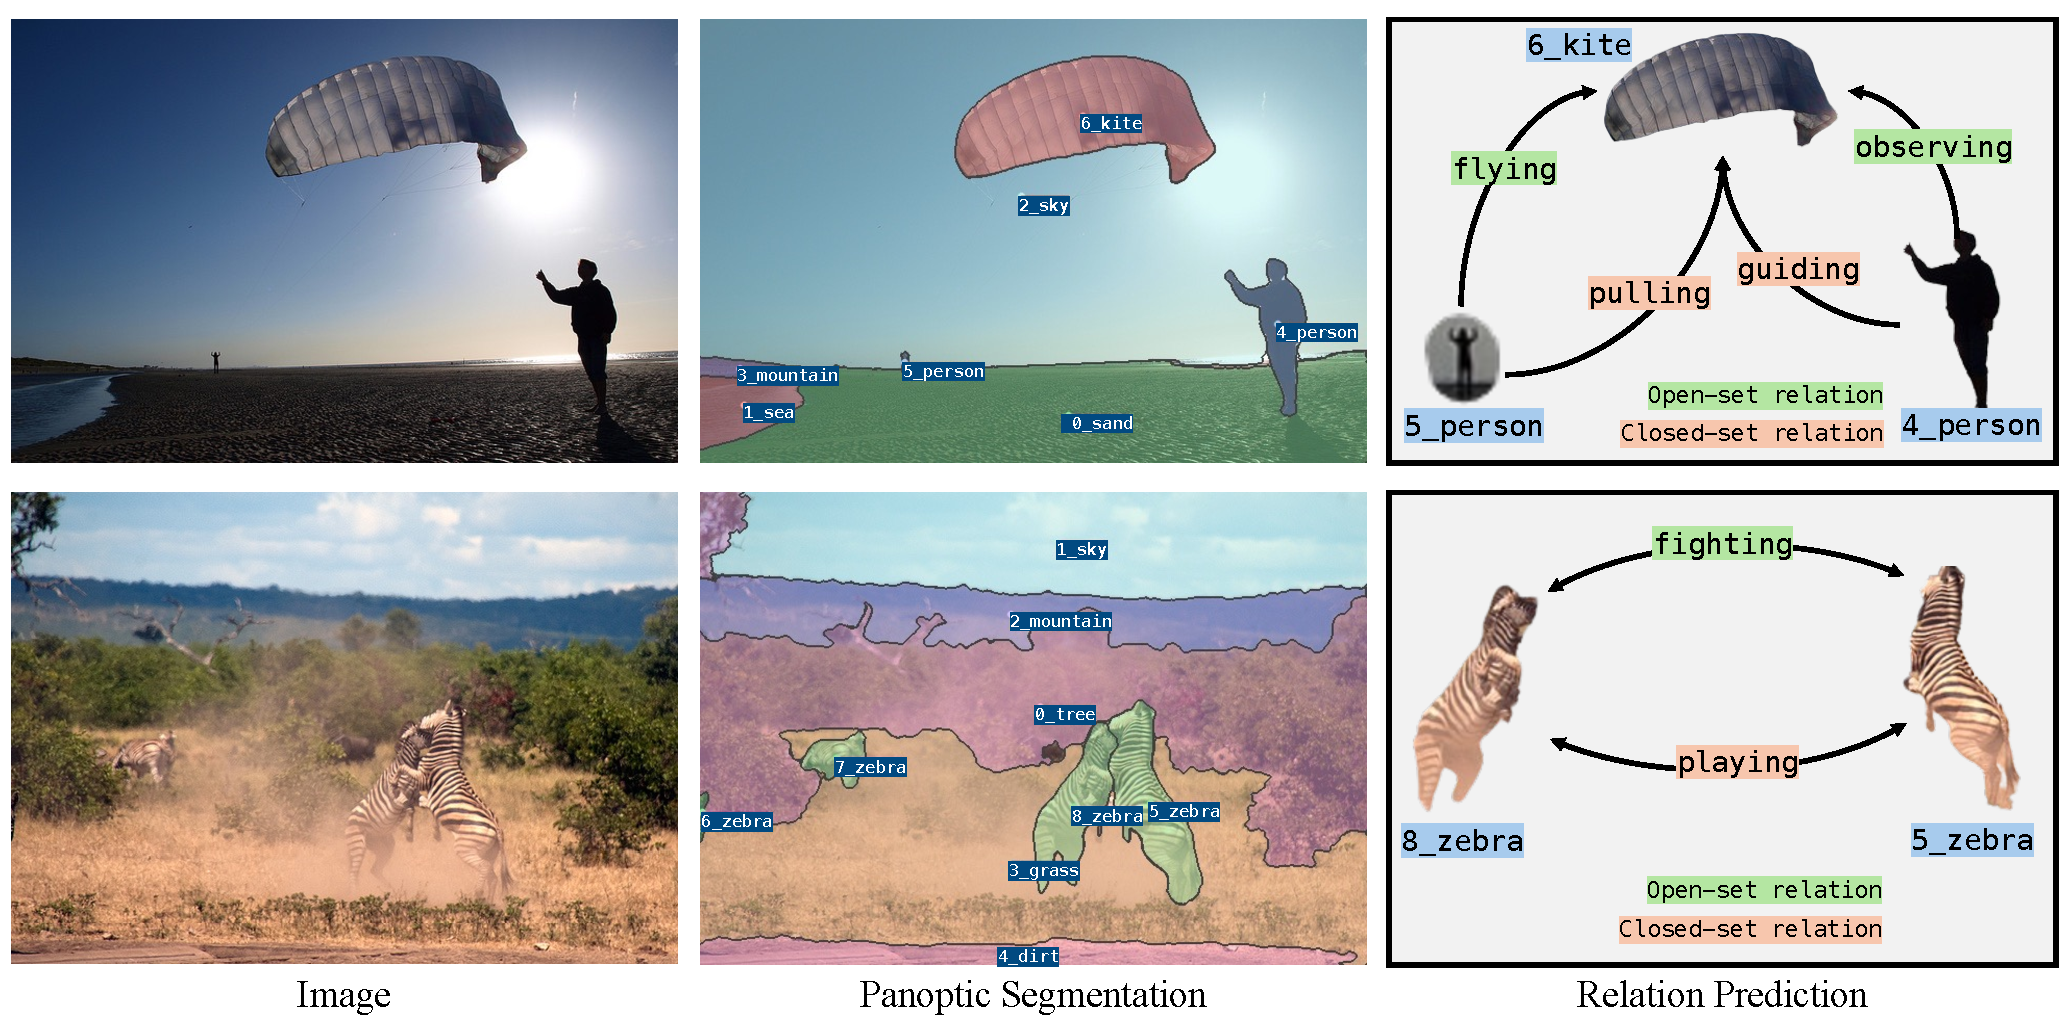
\includegraphics[width=1.0\linewidth]{Chapter5/Figures/vis2.pdf}
    \caption{Visualization results produced by our OpenPSG.
    The left image is the input to our OpenPSG, the middle one displays the panoptic segmentation result, and the right one shows the predicted relations between objects.
    }
    \label{openpsg:fig:vis2}
\end{figure}


\subsection{Visualization}
As shown in Fig.~\ref{openpsg:fig:vis2}, our OpenPSG method can predict relations not defined in the dataset, such as ``\textit{flying}'', ``\textit{observing}'', and ``\textit{fighting}'', which qualitatively demonstrates the excellent open-set relation prediction capability of our method.
